\documentclass[../jarvis.tex]{subfiles}
\usepackage{polynom}
\usepackage{scrambledenvs}
\newscrambledenv{hint}
\graphicspath{{\subfix{../images/}}}
\begin{document}
Outside of quadratic polynomials, there are also cubics, quartics, quintics, sextics..., that most students assume are extinct. However, they can be found in a select number of natural hideouts! In this handout, we look at the structures associated with polynomials, as well as the techniques to deal with them. 

\begin{figure}[H]
    \centering
    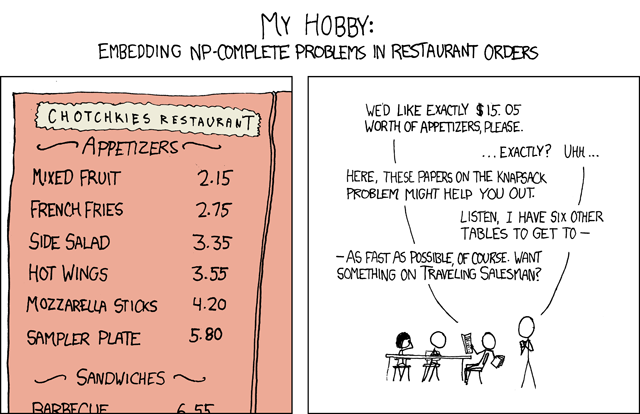
\includegraphics[scale=7]{xkcd_np_complete.png}
    \caption{Comic from https://xkcd.com/287/}
\end{figure}
\section{Quadratics \ez}
In this section, we will revisit the common quadratic polynomials.
The techniques for quadratics aren't many. The usual few are the discriminant and completing the square, none of which are totally unexpected or inspiring. However, they are still useful-ish in extracting information from a given problem.

\subsection{Algebraic Properties of Quadratics \ez}
We begin by stating some algebraic properties of the quadratic curve. In what follows, let $$P(x)=ax^2+bx+c=a\left(x+\frac{b}{2a}\right)^2+\left(c-\frac{b^2}{4a}\right).$$
\begin{proposition}[Quadratic Formula]
    The two (not necessarily distinct) roots of $P(x)$ is given by the \textit{quadratic formula}
    $$x=\frac{-b\pm\sqrt{b^2-4ac}}{2a}.$$
\end{proposition}
\begin{proof}
    Consider the completed square form, then 
    \begin{align*}
        P(x)=0 &\iff a\left(x+\frac{b}{2a}\right)^2+\left(c-\frac{b^2}{4a}\right)=0 \\
        &\iff a\left(x+\frac{b}{2a}\right)^2=\frac{b^2}{4a}-c \\
        &\iff \left(x+\frac{b}{2a}\right)^2=\frac{b^2-4ac}{4a^2} \\
        &\iff x+\frac{b}{2a}=\frac{\pm\sqrt{b^2-4ac}}{2a} \\
        &\iff x=\frac{-b\pm\sqrt{b^2-4ac}}{2a}
    \end{align*}
\end{proof}
\begin{proposition}[Discriminant]
    The discriminant is given by $\Delta=b^2-4ac$.
\end{proposition}
Observe that $\Delta$ lies under the square root in the numerator of the quadratic formula. Hence, if $\Delta>0$, there are two distinct roots. If $\Delta=0$, the root is simply $x=-\frac{b}{2a}$.

The special case is if $\Delta<0$, then we have two complex roots. This also says that complex roots come in \textit{conjugate pairs}, that is if
$$x_1=\frac{-b}{2a}\pm\frac{\sqrt{\abs{b^2-4ac}}}{2a}i$$
is a root, then so is
$$x_2=\frac{-b}{2a}\mp\frac{\sqrt{\abs{b^2-4ac}}}{2a}i.$$

\subsection{Geometric Properties of Quadratics}
The quadratic is also miraculous in that it is symmetric about it's \textbf{vertex}.

The graphical behaviour of a quadratic depends largely on its \textbf{leading coefficient}, that is the coefficient of the highest degree term. For $P(x)$, the leading coefficient is $a$.

Indeed, for large values of $x$, $P(x)$ is \textbf{dominated} by the term $ax^2$. If $a>0$, then $P(x)$ tends to positive infinity, that is, the graph opens \textbf{upwards}. On the other hand, if $a<0$, then $P(x)$ tends to negative infinity, that is, the graph opens \textbf{downwards}.

\begin{figure}
    \centering
    \begin{minipage}{.5\textwidth}
      \centering
      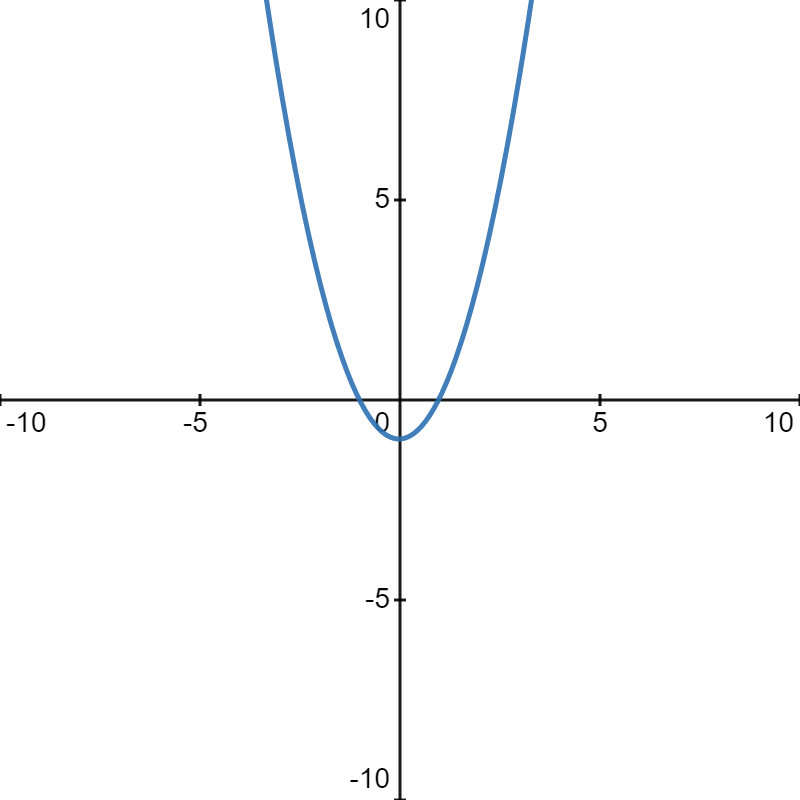
\includegraphics[width=.7\linewidth]{quadratic_up.png}
      \caption{For $a>0$.}
    \end{minipage}%
    \begin{minipage}{.5\textwidth}
      \centering
      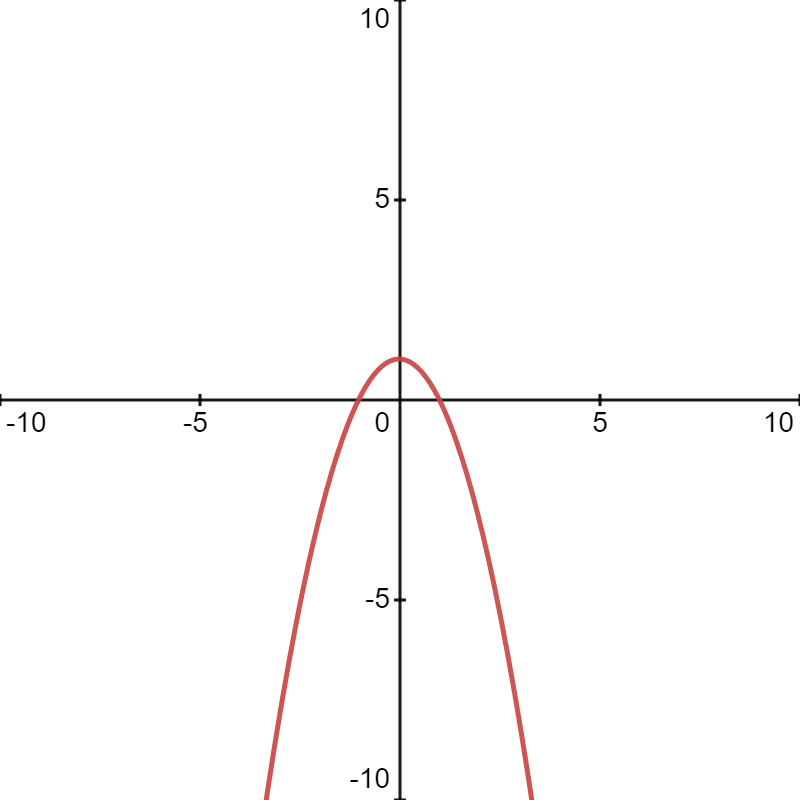
\includegraphics[width=.7\linewidth]{quadratic_down.png}
      \caption{For $a<0$.}
    \end{minipage}
\end{figure}

From the graph, one can also observe that the quadratic curve is \textbf{symmetric}. Crucially, it is symmetric about it's vertex, that is, the maximum or minimum point of the quadratic, depending on whether $a$ is positive or negative. We first discover the coordinates of the vertex.
\begin{proposition}[Coordinates of the Vertex]
    The vertex occurs at $x=\frac{b}{2a}$.
\end{proposition}
\begin{proof}
    Consider again the completed square form. Then,
   \begin{align*}
        P(x)&=a\left(x-\frac{b}{2a}\right)^2+\left(c-\frac{b^2}{4a}\right) \\
        &\geq c-\frac{b^2}{4a},
   \end{align*}
   because $\left(x-\frac{b}{2a}\right)^2\geq 0$. This leads us to the most important inequality for any polynomial: \textbf{the trivial inequality}.
   \begin{proposition}[The Trivial Inequality]
       For any real $x$, $x^2\geq 0$.
   \end{proposition}
   This is easily seen by considering the graph $y=x^2$, and noting that it is tangent to the line $y=0$. 
   
   Moreover, we make the crucial observation that \textbf{\textit{any} quadratic curve is simply a scaled and translated copy of the curve $y=x^2$}.

   This means that the minimum value of the quadratic is $y=c-\frac{b^2}{4a}$, and this value is achieved when $$\left(x-\frac{b}{2a}\right)^2=0 \implies x=\frac{b}{2a}.$$

   In other words, the coordinates of the vertex is $$\left(-\frac{b}{2a},c-\frac{b^2}{4a}\right).$$
\end{proof}
Moreover, the vertex is the point of symmetry. To illustrate, let $A$ and $C$ be two points that lie on the same horizontal line such that $A$ and $C$ are on different \textit{arms} of the curve. Then, the distance from $A$ to the line of symmetry and the distance from $C$ to the same line is equal.

In other words, $\abs{AB}=\abs{BC}$.
\begin{figure}[H]
    \centering
    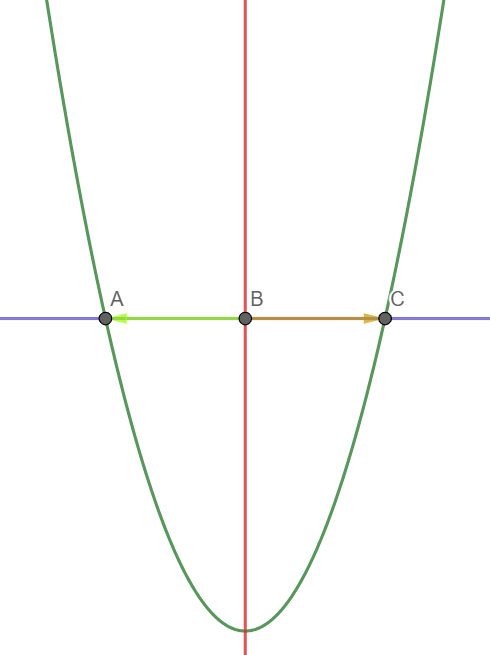
\includegraphics[scale=0.5]{quadratic_symmetry.PNG}
    \caption{Equidistance from the line of symmetry.}
\end{figure}

This property is independent of the constant term since the constant term only affects the \textit{upwards and downwards} shift of our quadratic graph. Hence, we shall ignore it and assume for convenience that the constant term is $0$. This means that for simplicity, we can simply assume that any quadratic curve has a vertex that lies exactly on the $x$-axis. And again, this is a legal assumption because the constant term does not affect our line of symmetry!

We now make use of our crucial observation that any quadratic is simply a scaled and translated version of $y=x^2$. Henceforth, let $Q(x)=\left(x-\frac{b}{2a}\right)^2$ (this is $P(x)$ without a constant term).

We note that the curve $y=x^2$ has a vertical line of symmetry at $x=0$. Thus, we obtain $Q(x)$ by \textbf{translating} the graph of $y=x^2$ by $\frac{b}{2a}$ units to the \textit{right} of the cartesian plane.

\begin{figure}[H]
    \centering
    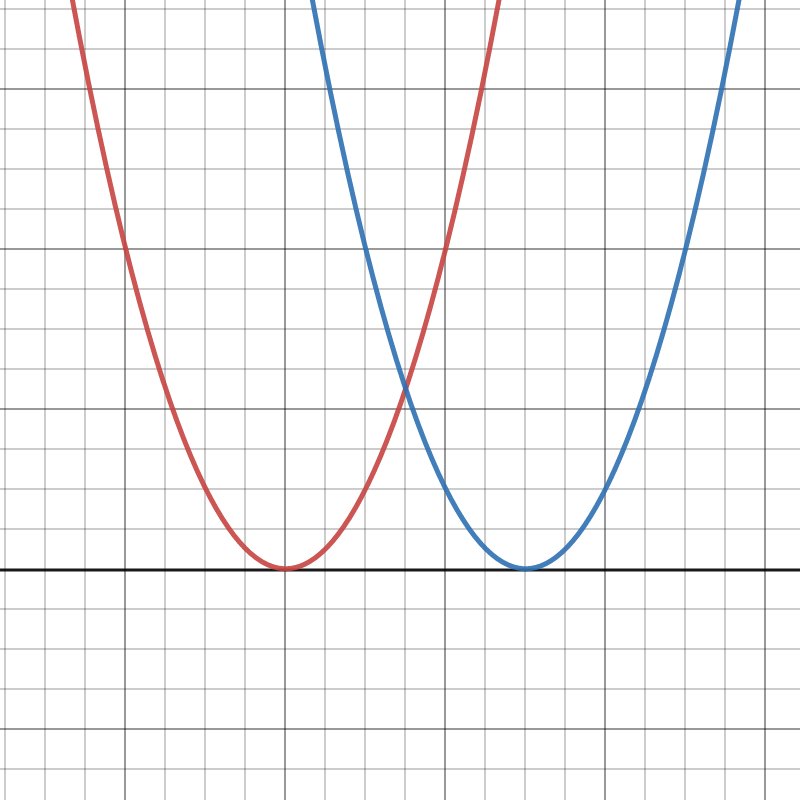
\includegraphics[scale=0.2]{quadratic_translate.png}
    \caption{$Q(x)$ (the blue curve) is obtained after translating $y=x^2$ (the green curve).}
\end{figure}

In formal terms, we say that $Q(x)$ is obtained by \textbf{translating} the graph of $y=x^2$ by $\frac{b}{2a}$ units \textbf{in the direction of the positive $x$-axis}. 

It is then a simple consequence of this symmetry that the $x$-coordinate of the vertex is the average of the roots of the quadratic. Indeed, let $r_1$ and $r_2$ be the roots, then
\begin{align*}
    r_1+r_2&=\left(-\frac{b}{2a}+\frac{\sqrt{\Delta}}{2a}\right)+\left(-\frac{b}{2a}-\frac{\sqrt{\Delta}}{2a}\right)=-\frac{b}{a}.
\end{align*}
\subsection{Roots of a Quadratic \ez}
With the basics and fundamentals out of the way, let us see how the algebraic and geometric properties play together nicely.
\begin{example}[2010-2011 Mandelbrot]
    Let $P(x)=x^3+ax^2+bx+c$ be a polynomial with three distinct roots. The polynomial P(Q(x)), where $Q(x)=x^2+x+2001$, has no real roots. Prove that $P(2001)>\frac{1}{64}$.
\end{example}
This is a strange idea: given the number of roots of a polynomial, what can we deduce about it's value?

\begin{proof}
    For starters, let $p,q,r$ be the three distinct roots of $P$, then $P(x)=(x-p)(x-q)(x-r)$ and let $z$ be a complex root of $P(Q(x))$ so that $P(Q(z))=0$. 

Hence, $Q(z)=\text{$p$ or $q$ or $r$}$. Without loss of generality, $$Q(z)=p \implies z^2+z+(2001-p)=0.$$

However, there are no real values of $z$ that satisfy this condition! This next step would be glaring: by considering the discriminant,
$$\Delta=1-4(2001-p) < 0 \implies p < \frac{8003}{4}.$$

Since we initially assumed without loss of generality that $Q(z)=p$, this conclusion should also hold for $q, r$, that is $p,q,r < \frac{8003}{4}$.

Finally, \begin{align*}
    P(2001)=(2001-p)(2001-q)(2001-r) &> \frac{1}{4}\cdot\frac{1}{4}\cdot\frac{1}{4} \\
    &=\frac{1}{64}
\end{align*}
\end{proof}
Next, we consider a quadratic with coefficients that form an arithmetic progression. As it turns out, if the quadratic has a unique root, then we can uniquely determine this root!
\begin{example}[2013 AMC 10B P19]
    Let $c,b,a$ be real numbers form an arithmetic progression with $a\geq b\geq c\geq 0$. The quadratic $ax^2+bx+c=0$ has exactly one root. Find this root.
\end{example}
First step! Our only root is $x=\frac{-b}{2a}$.

\begin{proof}
    Since $c,b,a$ have common differences with $b$ being the median element, we may write $c=2b-a$ so that 
$$b^2-4ac=b^2-4a(2b-a)=b^2-8ab+4a^2=0 \implies b=4a\pm2a\sqrt{3}.$$
Yet, we are given that $a\geq b$, so surely $b=4a-2a\sqrt{3}$, giving $x=-\frac{b}{2a}=\boxed{-2+\sqrt{3}}.$
\end{proof}

\section{Factor and Remainder Theorems \ez}
In what follows, we establish the idea that polynomials can be long divided, just as we can divide numbers. We first start with the "numbers" analog of division.

Suppose we want to divide $89$ by $3$, then trivially, $89=3\cdot 29+2$, where $3$ is the dividend, $29$ is the quotient and $2$ is the remainder. As it turns out, polynomials work in the same way!
\begin{proposition}[Division Algorithm for Polynomials]
    Let $f(x), d(x)$ be polynomials. Then, there exists polynomials $q(x)$ and $r(x)$ such that
    $$f(x)=d(x)\cdot q(x)+r(x),$$
    where $\deg r < \deg d$.
\end{proposition}
This can be proven by induction, which we defer to the end of this section.

From this result, we derive our two important theorems:
\begin{theorem}[Factor Theorem]
    $x-r$ is a factor of $P(x)$ \textbf{if and only if} $P(r)=0$.
\end{theorem}
\begin{theorem}[Remainder Theorem]
    $P(k)$ is the remainder when $P(x)$ is divided by $x-k$. 
\end{theorem}
\begin{remark}
    Note that the remainder theorem \textit{implies} the factor theorem!
\end{remark}

We start with an example on dividing polynomials.
\begin{example}[2011 SMO(O) P1]
    Let $S$ be the set of all integers $n$ $$\frac{8n^3-96n^2+360n-400}{2n-7}$$ is an integer. Find $\sum_{n\in S}\abs{n}.$
\end{example}
Damn, that's a big polynomial! But as the word "algorithm" in division algorithm suggests, we can do this systematically. 

We show two approaches, the first is a systematic approach which would be quick if you are confident with numbers, and the second is the standard long division. Either method works like a charm!

\textit{Approach 1:}
\paragraph{Step 1}We begin with the term of the largest degree, just as we begin from the digit with the largest value when long dividing integers.

To match the $8n^3$ term, we use $$4n^2(2n-7)=8n^3-28n^2\implies 8n^3=4n^2(2n-7)+28n^2.$$ This extra $n^2$ term is perfectly fine since we can simply defer it to the next step when we consider the quadratic term.

For now, we have 
\begin{align*}
    8n^3-96n^2+360n-400&=4n^2(2n-7)+28n^2-96n^2+360n-400 \\
    &=4n^2(2n-7)-68n^2+360n-400
\end{align*}

\paragraph{Step 2}We are done with dealing with the cubic term. Let us move on to the $n^2$ term now. To match the $-68n^2$ term, we use $$-34n(2n-7)=-68n^2+238n \implies -68n^2=-34n(2n-7)-238n.$$ Again, this extra $-238n$ term is fine.

Now, we have
\begin{align*}
    8n^3-96n^2+360n-400&=4n^2(2n-7)-68n^2+360n-400 \\
    &=4n^2(2n-7)-34n(2n-7)-238n+360n-400\\
    &=(2n-7)(4n^2-34n)+122n-400
\end{align*}

\paragraph{Step 3}Finally, we have the linear term in $122n$.
As again, we use $$61(2n-7)=122n-427 \implies 122n=61(2n-7)+427.$$ Then, 
\begin{align*}
    8n^3-96n^2+360n-400 &= (2n-7)(4n^2-34n)+122n-400 \\
    &= (2n-7)(4n^2-34n)+61(2n-7)+427-400 \\
    &= (2n-7)(4n^2-34n+61)+27.
\end{align*}
Now, we're home free!
\paragraph{Ending}
By factoring the common $(2n-7)$ terms, we get
$$8n^3-96n^2+360n-400=(2n-7)(4n^2-34n+61)+27.$$ 

\textit{Approach 2:}
\begin{center}
    \polyset{vars=XYZn}
    \polylongdiv{8n^3-96n^2+360n-400}{2n-7}
\end{center}
    
Now, we go back to our original problem: we wanted to divide by $(2n-7)$, so we do so:
$$\frac{8n^3-96n^2+360n-400}{2n-7}=4n^2-34n+61+\frac{27}{2n-7}.$$
This is the result of our polynomial \textit{long} division! It's simple, but it surely is long. In any case, we finish up the problem as such:

\begin{proof}
    We have that $$\frac{8n^3-96n^2+360n-400}{2n-7}=4n^2-34n+61+\frac{27}{2n-7}.$$
    For the fraction to be an integer, we require $2n-7\mid 27$ (this means that $2n-7$ divides 27). Thus,
    $$2n-7=\pm 1,\pm 3, \pm 9,\pm 27.$$
    This corresponds to $n=3,4,2,5,-1,8,-10,17$ only. Hence,
    $$\sum_{n\in S}\abs{n}=\boxed{50}.$$
\end{proof}

\begin{example}[2017 AMC12A P23]
    For certain real numbers $a,b$ and $c$, the polynomial
    $$g(x)=x^3+ax^2+x+10$$ has three distinct roots, and each root of $g(x)$ is also a root of the polynomial
    $$f(x)=x^4+x^3+bx^2+100x+c.$$
    Find $f(1)$.
\end{example}
This is a job for the factor theorem! ...if only we knew what the factors were. In any case, the problem implies that $g(x)$ is a factor of $f(x)$, and so we have
$f(x)=g(x)h(x)$ for some polynomial $h(x)$. But, since $f(x)$ is quartic and $g(x)$ is a cubic, $h(x)$ must be linear, so let $h(x)=x+r$ for some real $r$.

\begin{proof}
    Then, $$x^4+x^3+bx^2+100x+c=(x^3+ax^2+x+10)(x+r).$$
    Now, we should compare coefficients: there is nothing to work with for the quartic term, so we consider the $x^3$ term.
    
    Observe that on the right hand side, the only ways to contribute terms in $x^3$ is from $x^3\cdot r$ and $ax^2\cdot x$. This gives 
    $$1=r+a.$$
    Now, the quadratic term seems a bit messy, so we consider the linear term first: observe that the only ways to contribute terms in $x$ is $x\cdot r$ and $10\cdot x$, so
    $$100=10+r.$$
    Hence, $r=90$ and $a=-89$. 
    
    Finally, let us consider the quadratic term: the only ways to contribute terms in $x^2$ is $ax^2\cdot r$ and $x\cdot x$, so
    $$b=ar+1,$$
    but hmm, this is \textit{quite} big.
    
    When some numbers in our working gets a bit too big, it's usually a sign to relook our approach. In particular, what are we actually finding? We wanted $f(1)$,
    so $$f(1)=(1+a+1+10)(1+r)=-77\cdot 91=\boxed{-7007}.$$
\end{proof}

\begin{example}[2018 SMO(O) P16]
    Let $P(x)$ be a polynomial of degree $4$ such that $P(n)=\frac{120}{n}$ for $n=1,2,3,4,5$. Find the value of $P(6)$.
\end{example}
Firstly, we are told that the equation $nP(n)=120$ has 5 roots $n=1,2,3,4,5$. So, let us consider the polynomial
$$g(n)=nP(n)-120=C(n-1)(n-2)(n-3)(n-4)(n-5),$$
where $C$ is the leading coefficient of our expansion, and also the leading coefficient of $P(x)$.

We should first determine the value of $C$ (we know it's positive by comparing the constant coefficients). We substitute $n=0$ so that $$-120=C\left(-1\cdot-2\cdot-3\cdot-4\cdot-5\right) \implies C=1.$$
But wait, why are we allowed to do this? Isn't $P(0)$ undefined by since $P(n)=\frac{120}{n}$?

Seen in that way, it is. However, $g(n)$ is a polynomial in $n$, and since it is defined for all values other than at $n=0$ (by the given relation), then it must be defined at $n=0$ as well, since polynomials are continuous throughout!

Thus, $nP(n)-120=(n-1)(n-2)(n-3)(n-4)(n-5)$. Finally, $P(6)=\boxed{40}.$

In short, polynomial makes most things easy. In fact, it also makes maximising and minimising tidier (we are civilised people, so we don't differentiate).
\begin{example}[2019 SMO(S) P16]
    Let $M$ be the maximum possible value of $$\frac{15x^2-x^3-39x-54}{x+1},$$ where $x$ is an integer. Find $9M$.
\end{example}
Of course, we should long divide! I leave that to you:
$$\frac{15x^2-x^3-39x-54}{x+1}=-x^2+16x-55+\frac{1}{x+1}=(5-x)(x-11)+\frac{1}{x+1}.$$

Observe that $(5-x)(x-11)$ is positive for $5<x<11$ and let $y=x+1$, so 
    $$\frac{15x^2-x^3-39x-54}{x+1}=(6-y)(y-12)+\frac{1}{y}.$$
Then, this is positive for $6<y<12$. Since we seek positive values of $x$ (and hence $y$), manual checking shows that $y=9$ gives $M=\frac{82}{9}$, achieved at $x=8$.

Hence, $9M=\boxed{82}$.

Before we go further, we note that sometimes a polynomial is  hard to factorise, especially if it has high degrees or have large coefficients. The Rational Root Theorem is extremely useful to help us discover any potential linear factors and rational roots.
\begin{proposition}[Rational Root Theorem]
For a polynomial $P(x)=a_nx^n+a_{n-1}x^{n-1}+\cdots+a_1x+a_0$ with real coefficients $\{a_n\}=0$, if $P(x)$ \textit{has a rational root} $x=\frac{p}{q}$ where $\gcd(p,q)=1$, then
\begin{itemize}
    \item $p$ is an integer factor of the constant term $a_0$, and
    \item $q$ is an integer factor of the leading coefficient $a_n$.
\end{itemize}
\end{proposition}
It is important to point out that this \textbf{does not} guarantee that $P(x)$ has a rational root. It merely proposes that there are candidates.

Let us see it in action.
\begin{example}[2011 AIME I/9]
    Suppose $x$ is in the interval $[0,\frac{\pi}{2}]$ and $$24\sin^3{x}=\cos^2{x}.$$
    Find $24\cot^2{x}$.
\end{example}
\begin{proof}
    We have $$24\sin{x}=24\cdot\frac{\cos^2{x}}{\sin^2{x}}=\cot^2{x}$$, so we simply need to find $24\cot^2{x}=576\sin{x}$.

    Again, $$24\sin^3{x}=\cos^2{x}=1-\sin^2{x} \implies 24\sin^3{x}+\sin^2{x}-1=0.$$

    By rational root theorem, the possible roots of the polynomial $24t^3+t^2-1=0$ are $$\pm 1,\pm \frac{1}{2},\pm \frac{1}{3},\pm \frac{1}{4},\pm \frac{1}{6},\pm \frac{1}{8},\pm \frac{1}{12},\pm \frac{1}{12}$$. This is a long list, but with some patience, we find that $t=\frac{1}{3}$ is a root. Hence, $$24t^3+t^2-1=(3t-1)(8t^2+3t+1).$$

    However, the quadratic $8t^2+3t+1$ has no real roots (check using the discriminant), and so our only root is $\sin{x}=t=\frac{1}{3}$. 

    Finally, $24\cot^2{x}=576\sin{x}=576\cdot\frac{1}{3}=\boxed{192}.$
\end{proof}

\section{Vieta's Theorem and Higher Ordered Polynomials \med}
Contrary to popular belief, there are higher degree polynomials in the wild. We first consider some identities associated with the coefficients of a general polynomial.

Consider a general polynomial $$P(x)=a_nx^n+a_{n-1}x^{n-1}+\cdots+a_1x+a_0$$ with real coefficients $\{a_n\}$. Then, the
\begin{enumerate}
    \item constant term is $P(0)$,
    \item sum of coefficients is $P(1)$,
    \item sum of \textit{odd-power} coefficients is $\frac{P(1)-P(-1)}{2}$,
    \item sum of \textit{even-power} coefficients is $\frac{P(1)+P(-1)}{2}$.
\end{enumerate}

The reader is strongly encouraged to derive the four properties above!

For the other coefficients, there are other higher-powered techniques (pun fully intended) to deal with them, but we will not introduce them here (for the interested, see the roots of unity filter).

We are guessing the student is familiar with the so-called "sum and product of roots" for a quadratic, and here, we introduce a generalisation - we have similar relations for higher-degree polynomials! This is given by Vieta's Theorem.

\begin{proposition}[Vieta's Theorem]
    A general polynomial $P(x)=a_nx^n+a_{n-1}x^{n-1}+\cdots+a_1x+a_0$ with real coefficients $\{a_n\}$ and real and complex roots $r_1, r_2, \cdots r_n$ has the following relations:
    \begin{align*}
        r_1+r_2+\cdots+r_n&=-\frac{a_{n-1}}{a_n}\\
        (r_1r_2+r_1r_3+\cdots+r_1r_n)+(r_2r_3+r_2r_4+\cdots+r_2r_n)+\cdots+r_{n-1}r_n&=\frac{a_{n-2}}{a_n} \\
        r_1r_2\cdots r_n=(-1)^n\frac{a_0}{a_n}
    \end{align*}
    In general, the \textit{sum of roots taken k at a time} is given by $(-1)^k\frac{a_{n-k}}{a_n}.$ Each of these sums are also known as \textit{elementary symmetric polynomials}.
\end{proposition}

At this point, it is only complete if we also derive some common algebraic identities and factorisations. 
\begin{proposition}[Classic]
    In what follows, assume the summation run over $x_1,x_2,\cdots,x_n$.
    \begin{enumerate}
        \item For the bivariate $x^2+y^2=(x+y)^2-2xy$, we also have the three-variable relation $$x^2+y^2+z^2=(x+y+z)^2-2(xy+yz+zx).$$
        In general, $$\left(\sum x_i\right)^2=\sum x_i^2-2\left(\sum_{1\leq i\leq q\leq n}x_ix_j\right).$$

        \item $x^3+y^3+z^3-3xyz=\frac{1}{2}(x+y+z)[(x-y)^2+(y-z)^2+(z-x)^2]$.
        This also implies $$x^3+y^3+z^3 \geq 3xyz,$$ because
        $(x-y)^2+(y-z)^2+(z-x)^2\geq 0$.
        \item Sophie-Germain Identity: $a^4+4b^4=(a^2+2b^2+2ab)(a^2+2b^2-2ab)$.
        \item Lagrange's Identity: $(a^2+b^2)(c^2+d^2)=(ac-bd)^2+(ad+bc)^2=(ac+bd)^2+(ad-bc)^2$
        \item $(a+b)^3-(a^3+b^3)=3ab(a+b)$.
        \item $(a+b)^5-(a^5+b^5)=5ab(a+b)(a^2+ab+b^2)$.
        \item $(a+b)^7-(a^7+b^7)=7ab(a+b)(a^2+ab+b^2)^2$.
    \end{enumerate}
\end{proposition}
\begin{example}[2016 SMO(O) P15]
    Let $p,q$ be integers such that the roots of the polynomial $f(x)=x^3+px^2+qx-343$ are real. Find the minimum value of $\abs{p^2-2q}$.
\end{example}
This question reeks of Vieta's theorem... With some foresight, we first derive a corollary of the AM-GM inequality for three variables. From identity 2, we know that
    $$x^3+y^3+z^3 \geq 3xyz.$$

    Now take $x=a^{\frac{2}{3}}, y=b^{\frac{2}{3}}, z=c^{\frac{2}{3}}$ so that
    $$a^2+b^2+c^2\geq 3\sqrt[3]{(abc)^2}.$$
    \textit{(whispers) This is a secret tool that will help us later!}
\begin{proof}
    
    Let $a,b,c$ be the real roots of $f$, then by Vieta's theorem, $p=-(a+b+c)$, $q=ab+bc+ca$, and $abc=343$.
    Thus,
    \begin{align*}
        \abs{p^2-2q}&=\abs{(a+b+c)^2-2(ab+bc+ca)} \\
        &=\abs{a^2+b^2+c^2} \\
        &\geq \abs{3\sqrt[3]{(abc)^2}} = \abs{3\sqrt[3]{343^2}} \\
        &=\boxed{147}
    \end{align*}
\end{proof}

\begin{example}[2001 All-Russian Olympiad]
    The equation $(x-\sqrt[3]{13})(x-\sqrt[3]{53})(x-\sqrt[3]{103})=\frac{1}{3}$ has three distinct roots $r,s,t$. Find the value of $r^3+s^3+t^3$.
\end{example}

First of all... yikes! Cube roots and cubes. However, it seems that the three cube roots look arbitrary: while the answer depends on their values, we can find an expression for $r^3+s^3+t^3$ in terms of these cube roots without caring about their values just yet. 
\begin{proof}
    We make the substitution $a=\sqrt[3]{13}$, $b=\sqrt[3]{53}$, $c=\sqrt[3]{103}$, so that our equation is transformed into $$(x-a)(x-b)(x-c)-\frac{1}{3}=0.$$ By Vieta's theorem, 
\begin{align*}
    r+s+t&=a+b+c \\
    rs+st+rt&=ab+bc+ca \\
    rst&=abc-\frac{1}{3}.
\end{align*}
Now, how do we use this to our advantage to find $r^3+s^3+t^3$? For starters, we may expand
$$(r+s+t)^3=r^3+s^3+t^3+3r^2s+3r^2t+3rs^2+3rt^2+3s^2t+3st^2+6rst.$$
We're close to finding something substantial - if we can simplify the sum of the terms in the form $m^2n$. A natural way to do this is to expand
$$(r+s+t)(rs+st+rt)=r^2s+r^2t+rs^2+rt^2+s^2t+st^2+3rst.$$

Aha! Now our expression simplifies nicely:
$$(r+s+t)^3=r^3+s^3+t^3+3(r+s+t)(rs+st+rt)-3rst,$$
whence upon arranging, we have
\begin{align*}
    r^3+s^3+t^3
    &=(\alpha+\beta+\gamma)^3-3(\alpha+\beta+\gamma)(\alpha\beta+\beta\gamma+\gamma\alpha)+3\left(\alpha+\beta+\gamma+\frac{1}{3}\right)\\
    &=(\alpha+\beta+\gamma)^3-3(\alpha+\beta+\gamma)(\alpha\beta+\beta\gamma+\gamma\alpha)+3(\alpha+\beta+\gamma)+1 \\
    &=\alpha^3+\beta^3+\gamma^3+1 \\
    &=\boxed{170}
\end{align*}
\end{proof}

\begin{example}[2019 AIME I P10]
For complex numbers $z_1, z_2,\cdots z_{673}$, the polynomial
$$(x-z_1)^3(x-z_2)^3\cdots(x-z_{673})^3$$
can be expressed as $x^{2019}+20x^{2018}+19x^{2017}+g(x)$ where $g(x)$ is a polynomial with complex polynomials and of degree \textit{at most} $2016$. Find the value of 
$$\sum_{1\leq j\leq k\leq 673}z_jz_k.$$
\end{example}
The sum requested of us is an elementary symmetric polynomial, so we would expect to use Vieta's theorem in some way.

Let $S, P$ denote the sum of roots one and twice at a time respectively and let $Q(x)$ denote the given polynomial. Note that the required sum is $P$. Since it's weird that the given polynomial is cubed throughout, we shall consider
$$p(x)=(x-z_1)(x-z_2)\cdots(x-z_{673})=x^{673}-Sx^{672}+Px^{671}+\cdots$$

Thus, $Q(x)=[p(x)]^3$. To find $S$ and $P$, we shall expand this to find the coefficients of $x^{2018}$ and $x^{2017}$. To do this quickly, we consider how terms in 3 products can be multiplied together to give the relevant terms.

To wit, 
\begin{enumerate}
    \item $x^{2019}$ can only be formed by multiplying all three $x^{673}$, and there is only 1 way to do this.
    \item $x^{2018}$ can be formed by multiplying two $x^{673}$ and one $Sx^{672}$, and there are $\binom{3}{1}=3$ ways to do this.
    \item $x^{2017}$ can be formed by multiplying two $x^{673}$ and one $Px^{671}$, and there are $\binom{3}{1}=3$ ways to do this. It can also be formed by multiplying one $x^{673}$ and two $Sx^{672}$, giving $3$ ways as well.
\end{enumerate}
\begin{proof}
    We now have,
\begin{align*}
    Q(x)=[p(x)]^3&=(x^{673}-Sx^{672}+Px^{671}+\cdots)(x^{673}-Sx^{672}+Px^{671}+\cdots)(x^{673}-Sx^{672}+Px^{671}+\cdots) \\
    &= x^{2019}-3Sx^{2018}+3(P+S^2)x^{2017}+g(x),
\end{align*}
and thus
$$\begin{cases} -3S=20 \\ 3(P+S^2)=19 \end{cases}\Rightarrow \begin{cases} S=-\frac{20}{3} \\ P=-\frac{343}{9}\end{cases}.$$

Hence, $\boxed{P=-\frac{343}{9}}$.
\end{proof}

For the final problem of this chapter, we shall prove identity 7.
\begin{example}[Classic]
    Factorise $(a+b)^7-(a^7+b^7)$.
\end{example}
\begin{proof}
    Certainly we need some observations to reduce this problem into a more tractable form. We note that $a=0$ or $b=0$ make the expression vanish, so $ab$ is a factor of the expression. Moreover, since the degrees on $a, b$ are odd, $a=-b$ also causes the expression to vanish. Thus, $a+b$ is also a factor.

    Thus, the expression is a polynomial that readily decomposes into the factor $ab(a+b)$ of degree $3$ and another factor of degree $4$ (or possibly more factors).

    Let $a,b,c$ be roots of the cubic with $c=-(a+b)$ such that
    $$\begin{cases}
        A&=a+b+c=0 \\
        B&=ab+bc+ca=-(a^2+b^2+ab) \\
        C&=abc=-ab(a+b)
    \end{cases},$$
    whence the cubic is $$x^3+Bx-C=(x-a)(x-b)(x-c).$$
    
    This gives $a^2+b^2+c^2=(a+b+c)^2-2(ab+bc+ca)=-2B$. We now "lift" the power up to $x^7$. Suppose $t$ is one of $a,b,c$. Thus, we have
    \begin{align}
        t^7&=t(C-Bt)^2=B^2t^3-2BCt^2+C^2t \\
        &=B^2(C-Bt)-2BCt^2+C^2t \\
        &=-2BCt^2+(C^2-B^3)t+B^2C \label{12-seventh}
    \end{align}
    Summing \eqref{12-seventh} over $t=a,b,c$,
    \begin{align*}
        a^7+b^7-(a+b)^7&=-2BC(-2B)+3B^2C\\
        &=7B^2C=-7ab(a+b)(a^2+ab+b^2)^2
    \end{align*}
    whence $$(a+b)^7-(a^7+b^7)=7ab(a+b)(a^2+ab+b^2)^2.$$
\end{proof}

\section{Optional: Smoothness, Continuity and Roots \med}
It would not be right if we fail to prove the most important property of a polynomial: polynomials are both \textbf{continuous} and \textbf{smooth}.

\subsection{Continuity and Smoothness}
We shall state the technical definitions of both terms and also outline a rudimentary proof of both properties.
\begin{definition}[Continuity]
    A function $f$ is said to be continuous at a point $c$ if 
    $$\lim_{x\rightarrow c}f(x)=f(c).$$
    In this vein, there are two conditions:
    \begin{enumerate}
        \item $f(c)$ is defined, and
        \item the left and right limits of $x\rightarrow c$ are equal.
    \end{enumerate}
\end{definition}
\begin{definition}[Smoothness]
    A function $f$ is said to be smooth if it has derivatives of all orders. In other words,
    $$f(x),f'(x),f''(x),\cdots$$
    all exist. 
    
    Such a function is also rightfully said to be of class $\mathbf{C}^{\infty}.$
\end{definition}
\begin{proposition}[Polynomials are continuous]
    Polynomials are continuous throughout.
\end{proposition}
\begin{proof}
    We make a few observations.
    \begin{enumerate}
        \item $f(x)=x$ is continuous everywhere.
        \item If $g(x)$ and $h(x)$ are continuous everywhere, then so is $g(x)h(x)$ by the algebra of limits.
        \item Hence, $x^n$ is continuous for all positive integer $n$.
        \item If $g(x)$ and $h(x)$ are continuous everywhere, then so is $g(x)+h(x)$ by the algebra of limits.
    \end{enumerate}
\end{proof}
\begin{proposition}[Polynomials are smooth]
    Polynomials are smooth throughout.
\end{proposition}
\begin{proof}
    This follows since polynomials are infinitely differentiable.
\end{proof}

The following problem showcases the idea of "pushing the limits". By that, we mean the useful property of limits: let $P$ be continuous throughout, then
$$\lim_{x\to a}P(x)=P\left(\lim_{x\to a}f(x)\right).$$

\begin{example}[2021 SMO(O) P6]
    Consider all polynomials $P(x,y)$ with two variables such that $P(0,0)=2020$ and for all $x$ and $y$, $P(x,y)=P(x+y,y-x)$. Find the largest possible value of $P(1,1)$.
\end{example}
It is always worthwhile to play around with special values of the polynomial before finally solving it. In any case, we should suspect that $P(1,1)=2020$ is our answer, as the constant polynomial $P\equiv 2020$ is a possible solution. While this is usually the case for an easily guessable problem, it is still wise to proceed carefully.

We begin with $P(1,1)$, then we have
$$\begin{cases}
    x+y&=1 \\
    y-x&=1
\end{cases} \implies y=1,x=0,$$ so $P(1,1)=P(1,0)$.

We also have that $x+y=1, y-x=0 \iff x=y=\frac{1}{2}$. Thus,
$$P(1,1)=P(1,0)=P\left(\frac{1}{2},\frac{1}{2}\right)=P\left(\frac{1}{4},\frac{1}{4}\right)=\cdots.$$ Now, the key claim is clear.
\begin{proof}
    We have, for all positive integer $n$, $$P(x,y)=P\left(\frac{x}{2^n},\frac{y}{2^n}\right).$$

    Since polynomials are continuous, we may take $n\to\infty$ whence $P(x,y)=P(0,0)$ for all $x,y$.

    Hence $P(1,1)=\boxed{2020}$.
\end{proof} 
It wouldn't be fair if we didn't also include a proof on the (not so) Fundamental Theorem of Algebra.
\begin{theorem}[Fundamental Theorem of Algebra]
    Every non-constant single-variable polynomial with complex coefficients has at least one complex root.
\end{theorem}
This is slightly different from our usual statement that a polynomial has $n$ real and complex roots, but as we shall see, both statements are actually equivalent! We begin with a \textit{lemma}:
\begin{lemma}[Maximum modulus principle]
Let $D$ be a closed disk of radius $r$ centered at the origin such that $\abs{p(z)}>\abs{p(0)}$ whenever $\abs{z}\geq r$. Since $D$ is compact, the minimum of $\abs{p(z)}$ on $D$ is thus achieved at some point $z_0$ in the interior of $D$.

Then, $p(z_0)=0$.
\end{lemma}
\begin{proof}
    We proceed by a proof by contradiction. Suppose for the sake of contradiction that $p(z_0)=a\neq 0$. Then, expanding about $z=z_0$, we get
    $$p(z)=a+c_k(z-z_0)^k+c_{k+1}(z-z_0)^{k+1}+\cdots+c_n(z-z_0)^n.$$ Here, $c_k$ are the coefficients of the polynomial after replacing $z$ with $z-z_0$ and expanding.

    For sufficiently close to $z_0$, 
    $p(z)\sim q(z)=a+c_k(z-z_0)^k.$ This means that $p(z)$ behaves asymptotically similar to $q(z)$.

    Hence,
    \begin{equation}\label{fta-bound}
        \frac{p(z)-q(z)}{(z-z_0)^{k+1}}\leq M
    \end{equation} for some positive $M$ in the neighbourhood of $z_0$. 
    
    Now, we wish to bound $p(z)$ in terms of $a$ and $M$. Our key ingredient is the root of unity: write $z-z_0=re^{i\theta}$ for some $\theta$. This traces a circle of radius $r$ about $z_0$, and so for a sufficiently small $r$ such that \eqref{fta-bound} holds,
    \begin{align*}
        \abs{p(z)}&=\abs{q(z)+p(z)-q(z)} \\
            &\leq \abs{q(z)}+r^{k-1}\abs{\frac{p(z)-q(z)}{r^{k+1}}}\\
            &\leq \abs{a+(-1)c_kr^ke^{ki\theta}}+Mr^{k+1} \\
            &=\abs{a}-\abs{c_k}r^k+Mr^{k+1}
    \end{align*}
    For a sufficiently small $r$, $\abs{a}-\abs{c_k}r^k+Mr^{k+1}<\abs{a}$, contradicting our definition of $\abs{p(z_0)}$.
\end{proof}
Hence, for a complex $z_0$ satisfying our definition, it is a root of $p(z)$. Now, by repeated long division, $p(z)$ has $n$ (real and) complex roots.

\section{Exercises}
\subsection{Warmup}
\problem[2012 SMO(S) P12]Find the sum of all positive integers $x$ such that $$\frac{x^3-x+120}{(x-1)(x+1)}$$ is an integer.
\problem[2018 SMO(S) P8]The polynomial $p(x)=x^3+Ax^2+Bx-3$ has a factor $x^2+7x+1$. Find the remainder when $p(x)$ is divided by $x-4$.
\problem[2021 SMO(S) P9]A quadratic polynomial $P(x)=ax^2+bx+c$ with $a\neq 0$ has the property that
$$P(n)=\frac{1}{n^2} \quad\text{for all}\quad n=-1,2,3.$$
Find the smallest positive value $k$ where $k\neq 2,3$ such that $P(k)=\frac{1}{k^2}$.
\problem[2021 SMO(S) P24]Let $n$ be a positive integer such that
$$\frac{2021n}{2021+n}$$ is also a positive integer. Find the smallest positive value $n$.
\problem[2018 SMO(O) P8]For $x>2017$, find the minimum value of $$\frac{x^2+x+2018}{x-2017}.$$
\problem[2019 SMO(O) P5]Let $(-1,0)$ lie on the curve $y=ax^2+bx+c$, where $a,b,c$ are three fixed reals not exceeding $\frac{1}{2}$. If the inequality $x\leq ax^2+bx+c\leq \frac{1}{2}(x^2+1)$ holds for all real $x$, find the value of $2020(a^2+b^2-c^2)$.
\begin{hints}
    \begin{hint}
        Apply the discriminant on both side of the given inequality.
    \end{hint}
\end{hints}
\subsection{Problems}
\problem[2019 SMO(O) P8]Among all reals $a,b,c$ satisfying $a+b+c=0$ and $abc=10$, find the largest possible value of $a^3+b^3+c^3$.
\begin{hints}
    \begin{hint}
        Apply one of the identities found under Vieta's Theorem.
    \end{hint}
\end{hints}
\problem[2018 SMO(O) P11]Find the shortest distance from the point $(22,21)$ to the graph with equation $x^3+1=y(3x-y^2)$.
\begin{hints}
    \begin{hint}
        Apply one of the identities found under Vieta's Theorem.
    \end{hint}
    \begin{hint}
        This is identity 2, for what choice of $z$ would it be convenient? 
    \end{hint}
\end{hints}
\problem[2021 SMO(O) P9]Find the largest possible value of $a^4+b^4+c^4$ among all possible sets of $(a,b,c)$ satisfying
\begin{align*}
    a+b+c&=2\\
    a^2+b^2+c^2&=14\\
    a^3+b^3+c^3&=20
\end{align*}
\begin{hints}
    \begin{hint}
        Find $a+b+c$, $ab+bc+ca$ and $abc$.
    \end{hint}
    \begin{hint}
        Find a cubic equation that $a,b,c$ satisfies.
    \end{hint}
\end{hints}

\subsection{Challenges}
\problem[2014 SMO(O) P3]Consider the quadratic polynomial $g(x)=Ax^2+Bx$, where $A$ and $B$ are constants. Suppose $u$ and $v$ are two real numbers such that $$g(u-3)=g(v+3), \quad u-v\neq 6.$$
Find the largest possible value of $A(g(u+v))^2+B(g(u+v))$.\problem[2020 SMO(O) P16]Determine the smallest integer $p$ such that the system
$$\begin{cases}
    6x+4y+3z&=0 \\
    4xy+2yz+pxz&=0
\end{cases}$$
has more than one set of real solutions in $x,y,z$.
\begin{hints}
    \begin{hint}
        Begin by making a substitution into equation 2.
    \end{hint}
\end{hints}
\problem[2017 SMO(O) P16]There are $674$ apples, $674$ oranges and $674$ pears to be packed into $2$ boxes such that both boxes contains $3$ types of fruits and the products of the number of apples, pears and oranges in both boxes are the same. Determine the number of ways this can be done.
\begin{hints}
    \begin{hint}
        This is in fact an algebra problem! Define variables that represent the number of each type of fruits found in the first and second box.
    \end{hint}
    \begin{hint}
        Make a divisibility argument. You may wish to know that $337$ is prime.
    \end{hint}
\end{hints}

\problem[2017 SMO(O) P17]Let $S$ be the set of integers $x$ satisfying $2017x^2+(4036x-1)y+2019y^2=0$ for some integer $y$. Find the sum of all elements in $S$.
\begin{hints}
    \begin{hint}
        Notice that $2017+2019=4036$. Can we factorise part of the equation?
    \end{hint}
    \begin{hint}
        Substitute $z=x+y$.
    \end{hint}
    \begin{hint}
        Another divisibility argument! Look out for things that are coprime.
    \end{hint}
\end{hints}
\section{Hints to Exercises}
\printhint
\section{Solutions to Selected Problems}
\paragraph{2014 SMO(O) P3}
We have
\begin{align*}
    g(u-3)=g(v+3) &\iff A(u-3)^2+B(u-3)=A(v+3)^2+B(v+3) \\
    &\iff A(u^2-6u+9)+B(u-3)=A(v^2+6v+9)+B(v+3)\\
    &\iff A(u^2-v^2)-6A(u+v)+B(u-v)-6B=0 \\
    &\iff A(u+v)((u-v)-6)+B(u-v-6)=0 \\
    &\iff (A(u+v)+B)(u-v-6)=0.
\end{align*}
Since $u-v\neq 6$, $u+v=-\frac{B}{A} \implies g(u+v)=0$. Thus,
$$A(g(u+v))^2+B(g(u+v))=g(g(u+v))=g(0)=\boxed{0}.$$
\paragraph{2020 SMO(O) P16}Since the equations
$$\begin{cases}
    6x+4y+3z&=0 \\
    4xy+2yz+pxz&=0
\end{cases},$$
have more than one set of real solutions, we expect at least one variable to be the free variable, say $x$. That is, we may express $y,z$ in terms of $x$.
\begin{align*}
    4y=-6x-3z &\iff x(-6x-3z)+\frac{z(-6x-3z)}{2}+pxz=0 \\ &\iff 12x^2+(12-2p)xz+3z^2=0. \\
\end{align*}
This is a quadratic equation in terms of $x$, so
$$\Delta_{x}=(12-2p)^2z^2-144z^2=(12-2p)^2z^2-144z^2\geq 0.$$

Hence, 
$$(12-2p)^2-12^2\geq 0 \implies -2p(24-2p)\geq 0,$$
giving $p\leq 0$ or $p\geq 12$.

We now show that $p=12$ suffices. Firstly, $x,z$ are related by the quadratic $$12x^2-12xz+3z^2=0 \implies 3(2x-z)^2=0 \implies z=2x.$$
Substituting these results into the first equation gives the solution $(x,y,z)=(t,-3t,2t)$ for all real $t$, which satisfies the second equation.

Hence, $p=\boxed{12}$ is the required integer.

\paragraph{2017 SMO(O) P16}Let $a,b,c$ be the number of apples, oranges and pears respectively in the first box. Then, we seek the number of triples of $(a,b,c)$ satisfying $1\leq a,b,c\leq 673$
\begin{align*}
    abc=(674-a)(674-b)(674-c) \iff 2abc=674^3-674^2(a+b+c)+674(ab+bc+ca) \\
    \iff abc=4\cdot 337^3-2\cdot 337^2(a+b+c)+337(ab+bc+ca).
\end{align*}
This means that $337\mid abc$ and since $337$ is prime, at least one of $a,b,c$ is a multiple of $337$. However, since $a,b,c\leq 673$, one of $a,b,c$ is exactly $337$. Henceforth, suppose WLOG that $a=337$.

Thus, we have $b+c=674$, giving $673$ solutions. By symmetry, each of $b=337$ and $c=337$ also gives $673$ solutions. However, we have triple counted the solution $x=y=z=337$, so the number of solutions to our system, and equivalently, the number of ways for such an arrangement is $673\cdot 3-2=\boxed{2017}.$

\paragraph{2017 SMO(O) P17}We make the observation that $2017+2019=4036$, so we may rewrite the initial equation as
$$2017x^2+(4036x-1)y+2019y^2=0 \implies (x+y)(2017x+2019y)=y.$$

Define $d=x+y$, so $d(2017d+2y)=y \implies 2017d^2+2yd=y \implies y(1-2d)=2017d^2$. Now, we make the crucial observation that $1-2d$ and $d^2$ are relatively prime, that is, $\\gcd(1-2d,d^2)=1$.

To see this, we consider their greatest common divisor: $$\gcd(d^2, 1-2d)=\gcd(4d^2, 1-2d)=\gcd(4d^2+2d(1-2d), 1-2d)=\gcd(2d,1-2d)=1.$$

Thus, $1-2d\mid 2017$, but $2017$ is prime, so $1-2d=-1,1,-2017,2017$, giving $d=1,0,1009,-1008$. Correspondingly, $y=-2017,0,-1009^2,1008^2$ and $x=d-y=2018,0,1009+1009^2,-1008^2-1008$.

The sum is thus 
$$\sum_{S}=2018+(1009^2-1008^2)+(1009-1008)=2018+2017+1=\boxed{4036}.$$
\end{document}